\documentclass[a4paper,10pt,twoside,openany]{book}

\usepackage[lang=hebrew]{maths}
\usepackage{hebrewdoc}
\usepackage{stylish}
\usepackage{lipsum}
\let\bs\blacksquare

\setlength{\parindent}{0pt}

%%%%%%%%%%%%
% Styling %
%%%%%%%%%%%%

\usepackage{enumitem}

%%%%%%%%%%%%%
% Counters  %
%%%%%%%%%%%%%

\setcounter{section}{1}     
            
%BIBLIOGRAPHY
\usepackage[
backend=biber,
style=alphabetic,
]{biblatex}
\addbibresource{bibliography.bib} %Imports bibliography file

\title{
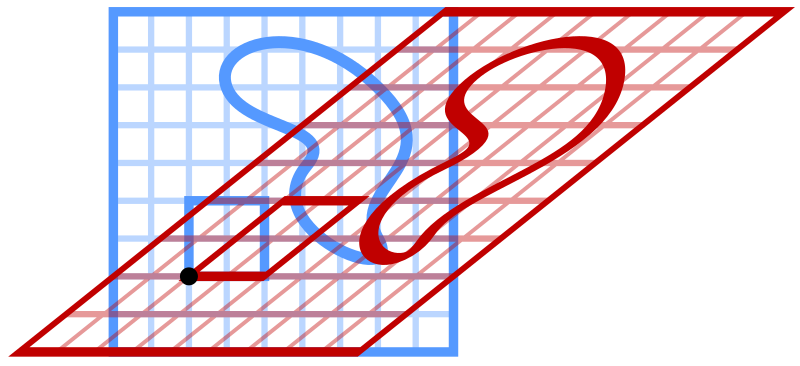
\includegraphics[width=6in]{images/front.png}\\
\vspace{30pt}
\Huge
מבוא לתורת המספרים (104157)
\\
אביב 2024
\\
רשימות תרגולים
\vspace{30pt}
\\
\huge
אלן סורני
\vspace{30pt}
\\
\Large
הרשימות עודכנו לאחרונה בתאריך ה־%
\today
}
\date{}

\begin{document}
\frontmatter
\maketitle
\tableofcontents

\mainmatter

\section*{סימונים}

\begin{itemize}
\item[-]
$\mbb{N} = \set{0, 1, 2, \ldots}$
אוסף המספרים הטבעיים.
\item[-]
$\mbb{N}_+ = \set{1, 2, 3, \ldots}$
אוסף המספרים הטבעיים החיוביים (כלומר, לא כולל אפס).
\item[-]
$\brs{n} = \set{1, \ldots, n}$.
\item[-]
$\floor{x}$
המספר הכי גדול שקטן או שווה ל־%
$x \in \mbb{R}$.
\item[-]
$\ceil{x}$
המספר הכי קטן שגדול או שווה ל־%
$x$.
\item[-]
\begin{align*}
\gcd\prs{a_1, \ldots, a_n} \\
\lcm\prs{a_1, \ldots, a_n}
\end{align*}
בהתאמה, המחלק המשותף הגדול ביותר של המספרים
$a_1, \ldots, a_n$,
והכפולה המשותפת המינימלית שלהם.
\end{itemize}

\chapter{תרגול 3 - שימושים בפריקות יחידה}

\section{תזכורת}

\begin{definition}
יהי
$n \in \mbb{N}_+$.
נגדיר
\begin{enumerate}
\item $\nu\prs{n} \coloneqq \sum_{d \mid n} 1$. זה מספר המחלקים של $n$.
\item $\sigma\prs{n} \coloneqq \sum_{d \mid n} d$. זה סכום המחלקים של $n$.
\item \[\text{.}\phi\prs{n} \coloneqq \sum_{\substack{\gcd\prs{d,n} = 1 \\ 1 < d < n}} 1\] זה מספר המספרים הטבעיים שקטנים מ־%
$n$
וזרים לו.
זאת נקראת
\textbf{פונקציית אוילר (\textenglish{Euer totient function})}.
\item $\pi\prs{n}$ מספר האיברים הראשוניים הקטנים או שווים ל־%
$n$.
זאת נקראת
\textbf{פונקציית המספרים הראשוניים (
\textenglish{prime-counting~function})}.
\item \[\mu\prs{n} = \begin{cases}
\prs{-1}^\ell & \text{\textenglish{$\forall p$ prime}}: p^2 \nmid n \\
0 & \text{otherwise}
\end{cases}\]
כאשר
$\ell$
מספר הראשוניים שמחלקים את
$n$.
זאת נקראת
\textbf{פונקציית מביוס (\textenglish{Möbius function})}.
\end{enumerate}
\end{definition}

\section{תרגילים}

\begin{exercisechap}[פרק 2, תרגיל 7]
הסיקו מתרגיל 6 כי
\[\ord_p\prs{n!} \leq \frac{n}{p-1}\]
וכי
\[\text{.} \sqrt[n]{n!} \leq \prod_{p \mid n!} p^{1 / \prs{p-1}}\]
\end{exercisechap}

\begin{exercisechap}[פרק 2, תרגיל 8]
השתמשו בתוצאת התרגיל הקודם כדי להראות שיש אינסוף ראשוניים.

\emph{רמז:}
הראו קודם שמתקיים
$\prs{n!}^2 \geq n^n$
לכל
$n \in \mbb{N}_+$.
\end{exercisechap}

\begin{exercisechap}[פרק 2, תרגיל 15]
הראו כי
\begin{enumerate}[label = (\alph*)]
\item לכל
$n \in \mbb{N}_+$
מתקיים
\[\text{.} \sum_{d \mid n} \mu\prs{n/d} \sigma\prs{d} = n\]
\item לכל
$n \in \mbb{N}_+$
מתקיים
\[\text{.} \sum_{d \mid n} \mu\prs{n/d} \sigma\prs{d} = n\]
\end{enumerate}
\end{exercisechap}

\begin{exercisechap}[פרק 2, תרגיל 18]
הראו כי
\[\text{.} \forall m,n \in \mbb{N}_+ : \phi\prs{n} \phi\prs{m} = \phi\prs{\gcd\prs{n,m}} \phi\prs{\lcm\prs{n,m}}\]
\end{exercisechap}

\begin{exercisechap}[פרק 2, תרגיל 19]
הראו כי
\[\text{.} \forall m,n \in \mbb{N}_+ : \phi\prs{mn} \phi\prs{\gcd\prs{m,n}} = \gcd\prs{m,n} \phi\prs{m} \phi\prs{n}\]
\end{exercisechap}

\begin{exercisechap}[פרק 2, תרגיל 20]
הראו כי
\[\text{.} \prod_{d \mid n} d = n^{\nu\prs{n} / 2}\]
\end{exercisechap}

\begin{exercisechap}[פרק 2, תרגיל 23]
יהי
$f \in \mbb{Z}\brs{x}$
ויהי
$\psi\prs{n}$
מספר הערכים
$f\prs{j}$
עבור
$j \in \brs{n}$
כך ש־%
$\gcd\prs{f\prs{j},n} = 1$.

\begin{enumerate}[label = (\alph*)]
\item הראו כי
$\psi\prs{n}$
פונקציה כפלית וכי
$\psi\prs{p^t} = p^{t-1} \psi\prs{p}$
לכל ראשוני
$p \in \mbb{N}_+$.

\item הסיקו כי
\[\text{.} \psi\prs{n} = n \prod_{p \mid n} \frac{\psi\prs{p}}{p}\]
\end{enumerate}

\end{exercisechap}

\printbibliography
\end{document}
